%----------------------------------------------------------------------------------------
%	PACKAGES AND OTHER DOCUMENT CONFIGURATIONS
%----------------------------------------------------------------------------------------

\documentclass[12pt]{article}
\usepackage{graphicx}
\usepackage[utf8]{inputenc}  
\usepackage[T1]{fontenc} 
\usepackage[top=1.5cm,bottom=1.5cm,left=1.3cm,right=1cm,asymmetric]{geometry}

\usepackage{amsfonts}
\usepackage{graphicx}
\usepackage{amsmath}
\usepackage{fancyhdr}
\usepackage{array,multirow,makecell}
\usepackage{cancel}
\usepackage{subfig}
\usepackage{wrapfig}
\setcellgapes{1pt}
\makegapedcells
\newcolumntype{R}[1]{>{\raggedleft\arraybackslash }b{#1}}
\newcolumntype{L}[1]{>{\raggedright\arraybackslash }b{#1}}
\newcolumntype{C}[1]{>{\centering\arraybackslash }b{#1}}


\usepackage{tikz}
\usetikzlibrary{arrows,automata,fit}

\pagestyle{fancy}
\renewcommand{\footrulewidth}{1pt}
\fancyhead[R]{\textit{Master MVA : Probabilistic graphical models}}
\fancyfoot[L]{\textit{}}
%\usepackage{unicode-math}
%\setmathfont{XITS Math}
%\setmathfont[version=setB,StylisticSet=1]{XITS Math}


%\geometry{hmargin=1.5cm,vmargin=2cm}   

\begin{document}
\section*{Latent dirichlet allocation for label modelling}
\section*{Thibaud Ehret \& Sammy Khalife}
\begin{figure}[!h]
\centering
\captionsetup{justification=centering,margin=2cm}
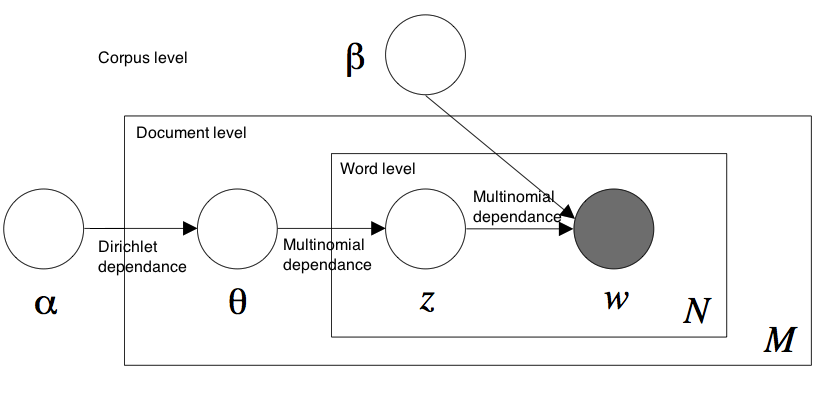
\includegraphics[width=15cm]{LDA.png}
\caption{Graphical model associated to LDA model}
\end{figure}
\begin{figure}[!H]
	\centering
	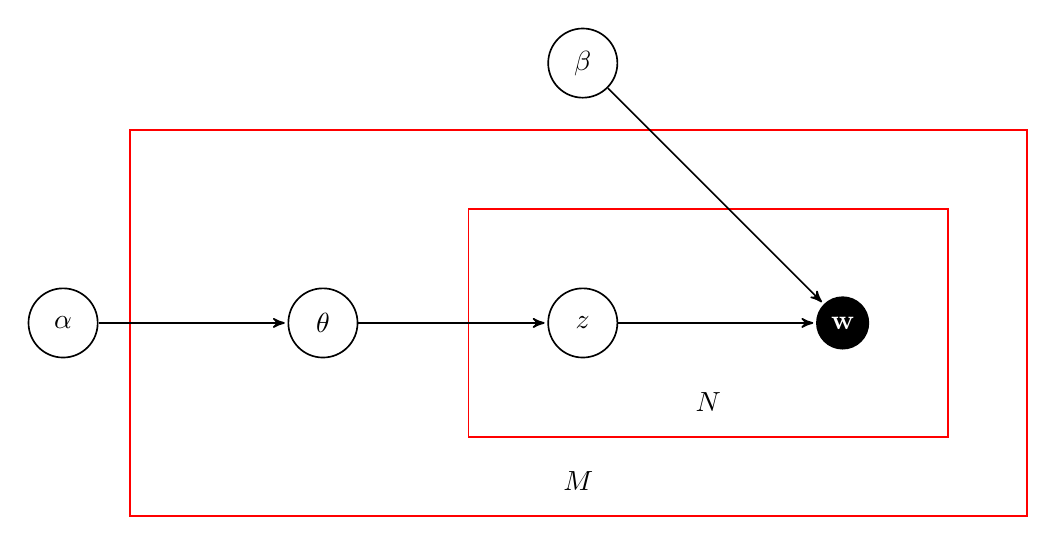
\begin{tikzpicture}[->,>=stealth',shorten >=1pt,auto,node distance=3.3cm,
		semithick]
		\tikzstyle{every state}=[fill=white,draw=black,text=black]
		\tikzstyle{final}=[circle, fill=black,draw=black,text=white]
		\node[state]         (A)                    {$\alpha$};
		\node[state]         (B) [right of=A]       {$\theta$};
		\node[state]         (C) [right of=B]       {$z$};
		\node[state]         (D) [above of=C]       {$\beta$};
		\node[final]         (E) [right of=C]       {$\textbf{w}$};
		\node (B1) [draw=red, fit= (E) (B) (C) , inner sep=2cm] {};
		\node (B2) [draw=red, fit= (C) (E), inner sep=1cm] {};
		\node [yshift=3.0ex, black] at (B1.south) {$M$};
		\node [yshift=3.0ex, black] at (B2.south) {$N$};
		\path (A) edge              (B)
	              (C) edge              (E)
	              (D) edge              (E)
	              (B) edge              (C);
	\end{tikzpicture}
	\caption{LDA model}
	\label{LDA_model}
\end{figure}


\begin{eqnarray*}
p(\textbf{w}|\alpha, \beta) &  = & \int p(\theta | \alpha, \beta)p(\textbf{w} | \alpha, \beta, \theta)d\theta\\
\end{eqnarray*}
In the LDA model, we have $ \theta \perp \beta$, and $p(w_{i} | \alpha, \beta, \theta) \perp p(w_{j} | \alpha, \beta, \theta)$  for $ i \neq j $
\begin{eqnarray*}
p(\textbf{w}|\alpha, \beta) & = & \int p(\theta | \alpha) \prod_{n=1}^{N} p(\textbf{w}_{n} | \alpha, \beta, \theta)d\theta\\
& = & \int  p(\theta |\alpha) \prod_{n=1}^{N}  \sum_{z_{n}}p(z_{n}|\alpha, \beta, \theta)p(\textbf{w}_{n} | \alpha, \beta, \theta, z_{n}) d\theta\\
\end{eqnarray*}
Moreover $z \perp (\alpha,\beta)$ and $\textbf{w}_{n} \perp (\alpha,\theta)$,
\begin{eqnarray*}
p(\textbf{w}|\alpha, \beta) & = & \int p(\theta | \alpha)  \prod_{n=1}^{N}  \sum_{z_{n}}p(z_{n} |\theta)p(\textbf{w}_{n} | z_{n}, \beta) d\theta\\
\end{eqnarray*}

\section{The algorithm}
We saw the complexity of the distribution associated to this model, therefore one can not simply calculate the posterior distribution for the inference and the parameter estimation. We will briefly present the algorithm used to calculate the inference and an approximation of the parameters. However, even if the distribution can not be computed, the algorithm is based on the EM principle.

\subsection{Inference}

The trick to be able to calculate the inference for the LDA model to calculate the variational inference which is a lower bound but easily calculable.

The lower bound is computed using the simplified graphical model presented in figure \ref{low_bound_model} which does not have the coupling between $\theta$ and $\beta$ and $\textbf{w}$.

The parameters $\gamma$ and $\phi$ for this new model are estimated by minimmizing the Kullback-Leibler divergence which has been shown to be good lower bound for the log-likelyhood. These are the parameters that we will use in the next part in order to estimate the parameters. 

\subsection{Parameter estimation}

We uses a modified version of the EM algorithm for this part. The expectation part, also called E-step, consists in computed the best variational parameters $\gamma$ and $\phi$ for the lower bound presented in the previous section. The maximization part, M-step, consists in optimizing the model parameter $\alpha$ and $\beta$ with the variational parameter fixed.
Just like in the EM algorithm, both step are then iterated until the bound of the model \ref{low_bound_model} converges.

\begin{figure}
	\centering
	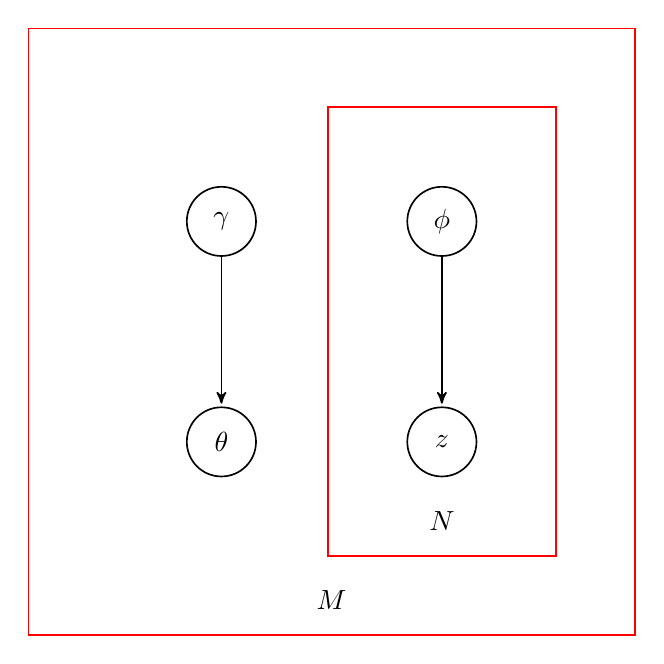
\begin{tikzpicture}[->,>=stealth',shorten >=1pt,auto,node distance=2.8cm,
		semithick]
		\tikzstyle{every state}=[fill=white,draw=black,text=black]
		\node[state]         (A)                    {$\gamma$};
		\node [state]        (B) [below of=A]       {$\theta$};
		\node[state]         (C) [right of=A]       {$\phi$};
		\node[state]         (D) [below of=C]       {$z$};
		\node (B1) [draw=red, fit= (A) (B) (C) (D), inner sep=2cm] {};
		\node (B2) [draw=red, fit= (D) (C), inner sep=1cm] {};
		\node [yshift=3.0ex, black] at (B1.south) {$M$};
		\node [yshift=3.0ex, black] at (B2.south) {$N$};
		\path (A) edge              (B)
	              (C) edge              (D);
	\end{tikzpicture}
	\caption{Graphical model used to calculate the lower bound of the log-likelyhood for the LDA graphical model}
	\label{low_bound_model}
\end{figure}

\section{Experiments}
Now that we have seeen how this model can be implemented in practice, we tried it on different type of data. The first type of data was 2 toy examples that we used in order to see how the algorithm would react in practice on data that we created and known to have a specific property so that we can expect some king of result and see if the result given by the code is actually the same than the one we could have been expecting. The second type of example was made using a real dataset called 20Newsgroups and try to analyze the result of the algorithm.

\subsection{Toy examples}

\subsubsection{First toy example}

The first toy example is simply a corpus made of 4 documents. Each of these documents containing a different word. We tried to find the repartition of the word into 4 different topics. The result that we were expecting was that the algorithm would put each word into its specific class just as this toy corpus seems to be doing. After running the algorithm we found the following result:

\begin{table}[ht]
	\centering
\begin{tabular}{c|c|c|c}
topic 1& topic 2& topic 3 & topic 4\\
\hline
word1	    & word2   &  word3          & word4\\
\end{tabular}
\caption{Table representing the result found by the model on the first toy example}
\label{tab1}
\end{table}

This result was exactly the one we were expecting which validates the mmodel for at least a really simple dataset.


\subsubsection{Second toy example}

The second toy example was not much complicated than the first one, but we wanted to see how the model would react on a slightly more complicated dataset but still easy enough so one could expect some result for the model. This second toy corpus is still made of 4 documents and overall contains 4 different words. This time two documents contain two words while the other two documents contains the two other words. We then try to find the repartition of the words into 2 topics. The result that we were expecting was that the two words being together in the same document would be in the same topic. After running the algorithm multiple time, we found two possible results that we present below:


\begin{table}[ht]
	\centering
\begin{tabular}{c|c}
topic 1& topic 2\\
\hline
word1 & word3\\
word2 & word4
\end{tabular}
\caption{Table representing one of the possible outcome of the algorithm on the second toy example}
\label{tab2}
\end{table}

\begin{table}[ht]
	\centering
\begin{tabular}{c|c}
topic 1& topic 2\\
\hline
word1 & word3\\
word2 & \\
word4 & \\
\end{tabular}
\caption{Table representing the second possible outcome of the algorithm on the second toy example}
\label{tab3}
\end{table}
The result presented in table \ref{tab2} being the result that we got for almost all the run but for one run we had the the result presented in table \ref{tab3}. While the result in table \ref{tab2} is exactly the one that we were expecting, the one presented in table \ref{tab3} could be considered wrong. This can show one of the limit of the algorithm which only maximizes a lower bound and therefore depending on the initialization we can have a wrong result for the model.

After having trieed on these easy example, we tried the model on a real dataset in order to be able to analyze the result.

\subsection{Experiment on a real dataset}

The dataset that we used is called 20Newsgroups and is made of approximatively 20000 documents that correspond to forums post from different language that can be classified into 6 major categories that are computers, hobbies, science, politics, religion and classified ads. Our idea was to run the algorithm with 6 topics on this corpus and analyze the classes that would be found by the model and see if these classes would make sense compared to the actual classes of the dataset. We present an extract of the result of the run of the algorithm on the full dataset in the following table:

\begin{table}[ht]
	\centering
\begin{tabular}{c|c|c|c|c|c}
topic 1& topic 2& topic 3 & topic 4 & topic 5 & topic 6\\
\hline
Atheism     & Foundation  & Archive    & Article&Journalism&Plastic\\
Atheist     & Telephone   & Galactic   & Edu &Disappointing&Prometheus\\
Religion    & Evolution   & Files      & Wolkswagon &Elysium&Citroen\\
Evolution   & Books       & Information& Autobahns &Madonna&Tractors\\
Chritians   & History     & Article    & Locomotive &Game&Wolkswagen\\
Bible       & Planets & Writes     & Motorway &&Bicycling\\
Biblical    & Newsletter  & Selection  & Sportscar &&Competitive\\
Clerical    & National    & Create     & Municipalities &&Window\\
Church      & Science     & Integrated & Shaman &&Thread\\
Christianity& National    & Goto       & Schoolteacher &&Course\\
Christian   & Magazine    & Xgif       &&&\\
Catholic    & Scientific  & Header     &&&\\
Christ      & Complex     & Panel      &&&\\
Theism      & Random      & Algorithmic&&&\\
Believer    & Silicon     &	       &&&\\
	    & Space       &            &&&\\
	    & Dinosaurs   &            &&&\\
\end{tabular}
\caption{Table representing an extract of the result found by the model on the 20Newsgroups dataset}
\label{tab4}
\end{table}

We will now try analyze the result given by the algorithm. First of all some of the categories can clearly be seen, such as religion for the topic 1, science for the topic 2 and computers for the topic 3. The last 3 topics are not as easy to analyze because of the lack of constitency in the whole topic. For example, when considering the 6th topic, one can see some words that would most likely appear in the science category such as Plastic, some words that could belong in the computer category like Window or Thread, some words that could belong in the hobby category like Bicycling or Competitive when talking about sport. One could therefore ask himself if there is actually a common structure behind all these words that the algorithm actually found a good topic for these words (we have to keep in mind that the model does only group into topics not necesseraly the one that we can see at first sight), even so it seems unlikely with the knowledge we have on these words and the possible contest one could have use them, or if this problem comes from the approximation, just like we saw in with the seecond toy example.





\end{document}
